% !TeX encoding = UTF-8 Unicode
% !TeX root = main.tex
% !TeX TS-program = pdflatex
%% (При смене движка необходимо удалить вспомогательные файлы *.aux *.brf *.log *.out *.synctex.gz *.toc)

\documentclass{thesisby}
\usepackage{etoolbox,ifxetex,ifluatex}
\usepackage[unicode,hypertexnames=false]{hyperref}

%%% Проверка используемого TeX-движка %%%
\ifboolexpr{bool{xetex} or bool{luatex}}{%
  \usepackage{fontspec}
  \PassOptionsToPackage{no-math}{fontspec}     % https://tex.stackexchange.com/a/26295/104425
  \usepackage{polyglossia}%[2014/05/21]        % Поддержка многоязычности

  % fonts and languages
  \defaultfontfeatures{Ligatures=TeX,Mapping=tex-text}

  \setmainlanguage[babelshorthands = true]{russian}
  \setotherlanguage{english}

  \setmainfont{Times New Roman}
  \setmonofont{Courier New}
  \setsansfont{Arial}

  \newfontfamily\cyrillicfont[Script=Cyrillic]{Times New Roman}
  \newfontfamily\cyrillicfontsf[Script=Cyrillic]{Arial}
  \newfontfamily\cyrillicfonttt[Script=Cyrillic]{Courier New}

  \newfontfamily\englishfont{Times New Roman}
  \newfontfamily\englishfontsf{Arial}
  \newfontfamily\englishfonttt{Courier New}

  \renewcommand{\UrlFont}{\small\rmfamily\tt}
}{%
  \usepackage[T1,T2A]{fontenc}
  \usepackage[utf8]{inputenc}
  \usepackage[english, russian]{babel}
  \usepackage{csquotes}
  \IfFileExists{pscyr.sty}{\usepackage{pscyr}}{}  % Подключение pscyr
}

% Для борьбы с переполнениями за счет разреженных слов в абзаце
\emergencystretch=25pt

\usepackage{enumitem}

\usepackage[
    language = auto,        % Получение языка из babel.
    autolang = other,       % Многоязычная библиография.
    defernumbers = true,    % Раздельная нумерация.
    style = gost-numeric,
    maxnames = 10,
    movenames = false,
    sorting = ynt
]{biblatex} % To load multiple bib files.

% Библиографический список в соответствии с ГОСТ.
\makeatletter
\ltx@iffilelater{biblatex-gost.def}{2017/02/01}%
{\toggletrue{bbx:gostbibliography}%
    \renewcommand*{\revsdnamepunct}{\addcomma}}{}
\makeatother

% Общий список.
\addbibresource{bibtexbase.bib}

% Список публикаций соискателя.
\addbibresource{bibtex_my.bib}
\DeclareSourcemap{
    \maps[datatype=bibtex, overwrite]{
        \map{
            \perdatasource{bibtex_my.bib}
            \step[fieldset=KEYWORDS, fieldvalue=idzm, append]
        }
    }
}

% Счётчики.
\usepackage[figure,table]{totalcount}   % Счётчик рисунков и таблиц.
\usepackage{totcount}                   % Пакет создания счётчиков на основе последнего номера подсчитываемого элемента (может требовать дважды компилировать документ).
\usepackage{totpages}

\usepackage{microtype}

%for lists
\usepackage[ampersand]{easylist}
\ListProperties(Hide=100, Hang=false, Margin=0mm, Indent1=10.5mm, Indent2=15mm, Style*=-- ,
Style2*=$\bullet$ ,Style3*=$\circ$ ,Style4*=\tiny$\blacksquare$ )

\newenvironment{easylistNum}{
    \begin{easylist}
        \ListProperties(Hide1=0, Hang=false, Margin=0mm, Indent1=10.5mm, Indent2=15mm, Start1=1, Style*=, FinalMark={)})}
        {\ListProperties(Hide=100, Hang=false, Margin=0mm, Indent1=10.5mm, Indent2=15mm, Style*=-- , Style2*=$\bullet$ ,Style3*=$\circ$ ,Style4*=\tiny$\blacksquare$ )
    \end{easylist}}

\usepackage{amsmath, amssymb, amsfonts}
\usepackage{longtable, array}
\usepackage{graphicx, epsfig}

\usepackage{algorithm}        % Для вставки псевдокода
\usepackage{algpseudocode}    % Для вставки псевдокода

% Русская традиция начертания греческих букв
\usepackage{upgreek} % Прямые греческие ради русской традиции (в формулах записывается \alpha как \upalpha и т.д.)

\usepackage{siunitx}% For Celsium sign only

\begin{document}

\hypersetup{
    pdftitle = {НЕЙРО-СЕМАНТИЧЕСКОЕ УПРАВЛЕНИЕ ДЛЯ ЗАДАЧ АСУТП},
    pdfauthor = {Иванюк Дмитрий Сергеевич},
    pdfsubject = {Диссертация},
    pdfkeywords = {ТеХ, диссертация }
}

% !TEX encoding = UTF-8 Unicode
\begin{titlepage}

    \begin{center} \bfseries
        % Национальная академия наук Беларуси\\
        \bigskip
        % {Учреждение образования}
        \medskip

        {БЕЛОРУССКИЙ ГОСУДАРСТВЕННЫЙ УНИВЕРСИТЕТ}
    \end{center}
    \vspace{1cm}

    \noindent УДК 004.032.26 \\
    \vspace{1cm}

    \begin{center}
        {Иванюк \\ Дмитрий Сергеевич}\\
        \vspace{1cm}

        {\bfseries НЕЙРО-СЕМАНТИЧЕСКОЕ УПРАВЛЕНИЕ ДЛЯ ЗАДАЧ АСУТП}\\
        \vspace{2cm}
        Диссертация на соискание ученой степени\\
        кандидата технических наук\\
        \bigskip

        по специальности 05.13.17 -- Теоретические основы информатики
    \end{center}
    \vspace{3cm}

    \begin{tabbing}
        \hspace{8cm} \= \kill \>
        Научный руководитель \+ \\
        доктор технических наук, профессор\\
        Головко В. А.
    \end{tabbing}


    \ifdefined\dissertationversion
        \vspace{3cm}
        \begin{center}
            \bfseries v\dissertationversion
        \end{center}
        \vspace{3cm}
    \else
        \vspace{7cm}
    \fi

    \begin{center}
        \bfseries Минск 2024
    \end{center}

\end{titlepage}


\tableofcontents

\chapter*{Перечень сокращений и обозначений}
\addcontentsline{toc}{chapter}{Перечень сокращений и обозначений}

\textit{ИНС} -- искусственная нейронная сеть

\textit{НС} -- нейронная сеть

\textit{АСУТП} -- автоматизированные системы управления технологическими процессами

\textit{ПИД} -- пропорционально-интегрально-дифференциальный регулятор

\textit{SCADA} -- (Supervisory for Control And Data Acquisition) система, обеспечивающая диспетчерское управление и сбор данных, относящаяся к классу программного обеспечения для создания АСУТП

\textit{«EasyServer»} -- SCADA-система, разработанная и применяемая на ОАО «Савушкин продукт» в АСУТП

\textit{PAC} -- Programmable Automation Controller - программируемый контроллер управления технологическим процессом

\textit{PFC} -- Programmable Fieldbus Controller - программируемый контроллер управления технологическим процессом

\textit{ОС} -- операционная система

\textit{ОУ} -- объект управления

\textit{ПОУ} -- пастеризационно-охладительная установка

\textit{OSTIS} -- Open Semantic Technology for Intelligent Systems, открытые семантические технологии для проектирования интеллектуальных -- гибкая, совместимая технология, обеспечивающая быстрое и качественное построение интеллектуальных систем различного назначения


\chapter*{Введение}
\addcontentsline{toc}{chapter}{Введение}

В современных условиях управление производством становится все сложнее, требования к эффективности более высокими. Задачи, находящиеся на уровне АСУТП, находятся в тесном взаимодействии как с верхним уровнем (планирование производства и т.п.), так и с нижним (уровень технологического оборудования). Один из путей улучшения производства может заключаться за счет совершенствования применяемых на уровне АСУТП подходов к управлению – применению последних разработок в данной области, одной из которых является нейроуправление.

ПИ- и ПИД-регуляторы были одними из первых систем управления \cite{Omatu_Khalid_Yusof}. Они зарекомендовали себя как относительно простые и надежные системы, которые достаточно эффективно решали поставленные задачи. И в настоящее время они остаются преобладающими системами управления, несмотря на наличие в них определенных недостатков и ограничений, которых лишено нейроуправление. Новые подходы позволяют строить более эффективные системы управления по сравнению с классическими ПИД-регуляторами.

Нейроуправление – относительно молодое направление научных исследований, которое стало самостоятельным в 1988 году. Однако исследования в этой области начались гораздо раньше. Одно из определений науки «кибернетика» рассматривает ее как общую теорию управления и взаимодействия не только машин, но и биологических существ. Нейроуправление пытается реализовать данное положение через построения систем управления (систем принятия решений), которые могут обучаться во время функционирования, и таким образом, улучшать свою эффективность работы. При этом такие системы используют параллельные механизмы обработки информации, подобно мозгу живых организмов \cite{Uskov_2004}.

Долгое время была популярна идея построения совершенной системы управления – универсального контроллера, который извне выглядел бы как «черный ящик». Он мог бы использоваться для управления любыми системами, имея связи с датчиками, исполнительными механизмами, другими контроллерами и специальную связь с «модулем эффективности» – системой, которая определяет эффективность управления исходя из заданных критериев. Пользователь такой системы управления задавал бы только желаемый результат, далее обученный контроллер управлял бы самостоятельно, возможно придерживаясь сложной стратегии достижения в будущем желаемого результата. Также он бы все время корректировал свое управление исходя из реакции объекта управления для достижения максимальной эффективности. Общая схема такой системы приведена ниже.

\begin{figure}[H]
    \tikzset{
        box/.style={
                % The shape:
                rectangle,
                % The size:
                minimum size=20mm,
                % The border:
                very thick,
                draw=red!50!black!50,         % 50% red and 50% black,
                % and that mixed with 50% white
                % The filling:
                top color=white,              % a shading that is white at the top...
                bottom color=red!50!black!20, % and something else at the bottom
                % Font
                font=\itshape,
                align=center}}

    \tikzset{big_arrow/.style={-{Stealth[length=5mm, width=4mm]}}}

    \centering
    \usetikzlibrary {positioning,shapes.misc,calc,arrows.meta,arrows}
    \begin{tikzpicture}[
            right1/.style={to path={-- ++(5,0) |- (\tikztotarget)}},
            left1/.style={to path={-- ++(-5,0) |- (\tikztotarget)}}]
        \node (o1)   [box]                        {Объект\\управления};
        \node (u1)   [below=of o1,align=center]   {$\mathbf{ U(t) }$\\Эффективность};
        \node (c1)   [box,below=of u1]            {Управляющее\\устройство\\(контроллер)};

        \node (control) [right=of c1,align=center]  {$\mathbf{ u(t) }$\\Управление};
        \node (sensors) [left=of c1,align=center]   {$\mathbf{ X(t) }$\\Показания датчиков};

        \path {
            (o1)            edge[very thick]                     (u1)
            (u1)            edge[very thick, big_arrow]          (c1)
            ($ (c1.east) $) edge[very thick, big_arrow, right1]  ($ (o1.east) $)
            ($ (o1.west) $) edge[very thick, big_arrow, left1]   ($ (c1.west) $) };
    \end{tikzpicture}

    \caption{Система с подкрепляющим обучением}
    \label{fig:reinforce_learning_system}
\end{figure}

В настоящее время не только оборудование, применяемое на ОАО «Савушкин продукт», характеризуется очень высокой сложностью, но и технологические процессы также. Настройка параметров технологических линий требует наличия специалистов высокого уровня и занимает длительное время. Соответственно требования к качеству изготовления продукции очень высоки, так как от него напрямую зависит размер получаемой прибыли (выше качество – лучше потребительские характеристики товара – дольше срок хранения – более широкие возможности по географическому охвату рынка и т.д.). Нейроуправление позволяет повысить качество продукции за счет повышения эффективности управления, а также ускорить настройку параметров. Поэтому актуальной является задача применения нейроуправления для построения сложных управляющих систем на уровне АСУТП, которые были бы лишены недостатков, присущих используемым системам (на основе ПИД-регуляторов).

\include{description_of_work}

\chapter{Современные системы управления}

Современные технологические процессы повышают требования для качества управления. Исследователи применяют для решения задач в данной области множество методов, в том числе искусственные нейронные сети, имеющие высокий потенциал в этой области. Однако они не обеспечивают значимых преимуществ перед классическими подходами и требуют улучшения.
В данной главе рассматриваются современные технологии и методы, применяемые в системах управления технологическими процессами, оценивается их эффективность и недостатки. Определены исходные данные для анализа и параметры качества. Выполнена постановка задачи исследования.

\section{ПИД-регуляторы}

ПИД-регуляторы доказали свою эффективность в управлении разнообразными процессами. Их использование не требует знания точной модели процесса, поэтому они эффективны в управлении промышленными и технологическими процессами, математические модели которых достаточно сложно определить. ПИД-регуляторы строятся на основе классической теории управления и просты для понимания и реализации (рис. \ref{fig:PID_controller_scheme}).

\begin{figure}[H]
    \centering
    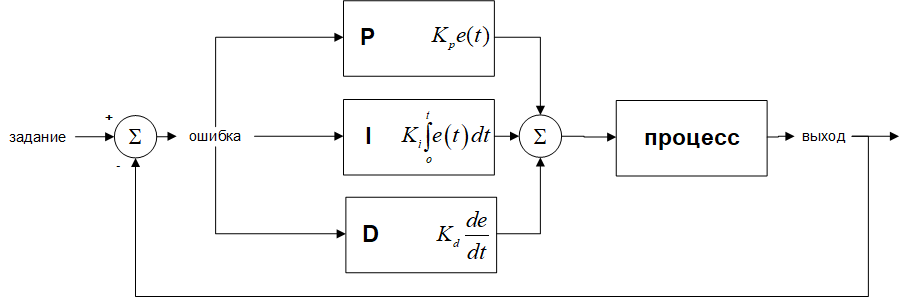
\includegraphics[width=\textwidth]{images/chapter1/Структурная схема ПИД-регулятора.png}
    \caption{Структурная схема ПИД-регулятора}
    \label{fig:PID_controller_scheme}
\end{figure}

\subsection{Описание ПИД-регуляторов}

Назначение ПИД-регулятора – в поддержании заданного значения $x_0$ некоторой величины $x$ с помощью изменения другой величины $u$. Значение $x_0$ называется заданием, а разность $e=(x_0-x)$ – невязкой или рассогласованием. Выходной сигнал контроллера $u$ определяется тремя слагаемыми:

\begin{equation}
    \label{eq_PID}
    u(t) = P + I + D = K_p e(t) + K_i \int_{0}^{t} e(t) dt + K_d \frac{de}{dt}
\end{equation}

где $K_p, K_i, K_d$ – коэффициенты усиления пропорциональной, интегральной и дифференциальной составляющих контроллера, соответственно.
Большинство методов настройки ПИД-регулятора используют несколько иную формулу для выходного сигнала, в которой на пропорциональный коэффициент усиления умножены также интегральная и дифференциальная составляющие:

\begin{equation}
    u(t) = K_p \left( e(t) + \frac{1}{T_i} \int_{o}^{t} e(\tau) d \tau +T_d \frac{de}{dt}\right).
\end{equation}

\textbf{Пропорциональная составляющая} – $K_p$ – вырабатывает выходной сигнал, который стабилизирует отклонение регулируемой величины. Выходной сигнал пропорциональной составляющей тем больше, чем сильнее регулируемая величина отклоняется от задания. Если входной сигнал равен заданию, то выходной равен нулю.

При использовании пропорционального контроллера значение регулируемой величины никогда не стабилизируется на заданном значении. Существует так называемая статическая ошибка, которая равна такому отклонению регулируемой величины, которое обеспечивает выходной сигнал, стабилизирующий выходную величину именно на этом значении. Например, в контроллере температуры выходной сигнал (мощность нагревателя) постепенно уменьшается при приближении температуры к заданию, и система стабилизируется при мощности равной тепловым потерям. Температура не может достичь задания, так как в этом случае мощность нагревателя станет равна нулю, и он начнет остывать.

Чем больше коэффициент пропорциональности между входным и выходным сигналом (коэффициент усиления), тем меньше статическая ошибка, однако при слишком большом коэффициенте усиления могут начаться автоколебания, а при дальнейшем увеличении коэффициента система может потерять устойчивость.

Для устранения статической ошибки используют \textbf{интегральную составляющую} – $K_i$. Она позволяет регулятору «учиться» на предыдущем опыте. Если система не испытывает внешних возмущений, то через некоторое время регулируемая величина стабилизируется на заданном значении, сигнал пропорциональной составляющей будет равен нулю, а выходной сигнал будет полностью обеспечивать интегральная составляющая.

\textbf{Дифференциальная составляющая} – $K_d$ – противодействует предполагаемым отклонениям регулируемой величины, которые могут произойти в будущем. Эти отклонения могут быть вызваны внешними возмущениями или запаздыванием воздействия регулятора на систему. Чем быстрее регулируемая величина отклоняется от задания, тем сильнее противодействие, создаваемое дифференциальной составляющей.

\subsection{Достоинства и недостатки ПИД-регуляторов}

Установление связей между параметрами и управление действиями системы может осуществляться инженерами-практиками и операторами.
Кроме того, за последние десятилетия разработано несколько методов настройки ПИД-регуляторов.

Однако, наряду с вышеуказанными достоинствами, ПИД-регуляторы имеют и ряд недостатков. Так, если рабочая точка процесса изменяется из-за возмущений, параметры контроллера требуется перенастраивать вручную, чтобы получить новую оптимальную настройку. Настройка должна осуществляться опытным оператором. Для систем с взаимодействующими контурами это процедура может быть сложной и занимать много времени. Кроме того, для процессов с переменными параметрами, временными задержками, существенными нелинейностями и значительными помехами использование ПИД-регуляторов может не обеспечить оптимальных характеристик.

Методы настройки ПИД-регуляторов также имеют ряд недостатков.
Одна из идей повышения эффективности ПИД-регуляторов заключается в управлении с самонастройкой, в котором параметры контроллера настраивались бы в оперативном режиме.

\subsection{Дискретная реализации ПИД-регулятора}

Идеализированное уравнение ПИД-регулятора (\ref{eq_PID}) является непрерывным, т. е. использует непрерывное время. При построении регулятора на базе компьютера входные и выходные переменные регулятора необходимо квантовать по времени с некоторым шагом $T_0$, и преобразовать в цифровую форму с помощью аналого-цифровых и цифро-аналоговых преобразователей. При этом уравнение ПИД-регулятора должно быть преобразовано в разностное с помощью замены производных конечной разностью, а интеграла – конечной суммой. В зависимости от выбранного метода перехода от непрерывных операторов к их дискретным аналогам возникает несколько различных уравнений, описывающих дискретные ПИД-регуляторы. При использовании метода прямоугольников для замены интеграла конечной суммой получим \cite{PID_NIL_AP}:


\begin{equation}
    \label{eq_discrete_PID}
    u(k) = K\left[ e(k) + \frac{T_0}{T} \sum_{i = 0}^{k} {e(i - 1)} + \frac{T_D}{T_0} (e(k) - e(k - 1))\right],
\end{equation}

где $k = 0, 1, \ldots\frac{t}{T_0}$ - порядковый номер отсчета дискретного времени.

Недостатком такого представления уравнения регулятора является необходимость помнить значения отклонений $e(k)$ для всех моментов времени от начала процесса регулирования.

Этот недостаток можно устранить, если для вычисления текущего значения управляющей переменной $u(k)$ использовать ее предыдущее значение $u(k-1)$ и поправочный член. Для получения такого рекуррентного алгоритма достаточно вычесть из уравнения (\ref{eq_discrete_PID}) следующее уравнение \cite{PID_NIL_AP}:

\begin{displaymath}
    u\left(k-1\right)=K\left[e\left(k-1\right)+\frac{T_0}{T}\sum_{i=0}^{k-1}{e(i-1)}+\frac{T_D}{T_0}(e\left(k-1\right)-e(k-2))\right].
\end{displaymath}

В результате получим [6]:

\begin{equation}
    u\left(k\right)-u\left(k-1\right)=q_0e\left(k\right)+q_1e\left(k-1\right)+q_2e\left(k-2\right),
\end{equation}

Где

\begin{equation}
    q_0=\mathbf{K}\left(1+\frac{T_D}{T_0}\right),
\end{equation}

\begin{equation}
    q_1=-\mathbf{K}\left(1+2\frac{T_D}{T_0}-\frac{T_0}{T_D}\right),
\end{equation}

\begin{equation}
    q_2=\mathbf{K}\frac{T_D}{T_0}.
\end{equation}

Таким образом, для вычисления текущего значения управляющего воздействия $u(k)$ на объект управления достаточно хранить в памяти только величины $u\left(k-1\right)$, $e\left(k\right)$, $e\left(k-1\right)$, $e(k-2)$, то есть величины

\begin{equation}
    u\left(k\right)=u\left(k-1\right)+\Delta u(k),
\end{equation}

\begin{equation}
    \Delta u\left(k\right)=q_0e\left(k\right)+q_1e\left(k-1\right)+q_2e\left(k-2\right).
\end{equation}

Итак, алгоритм работы ПИД-регулятора может быть представлен в следующем виде [3]:

\begin{equation}
    u\left(k\right)=u\left(k-1\right)+\Delta u(k),
\end{equation}

\begin{equation}
    \Delta u\left(k\right)=q_0e\left(k\right)+q_1e\left(k-1\right)+q_2e\left(k-2\right),
\end{equation}

\begin{equation}
    q_0=\mathbf{K}\left(1+\frac{T_D}{T_0}\right), q_1=-\mathbf{K}\left(1+2\frac{T_D}{T_0}-\frac{T_0}{T_D}\right), q_2=\mathbf{K}\frac{T_D}{T_0}.
\end{equation}

При переходе от непрерывных операторов к дискретным возникает погрешность, величина которой пропорциональна остаточному члену ряда Тейлора функции $e\left(t\right)$. Поэтому полученные дискретные уравнения можно считать эквивалентными непрерывным только при условии, что $e\left(t\right)$ изменяется слабо в пределах такта квантования. Однако с помощью аппарата z-преобразования можно показать, что основные свойства ПИД-регулятора сохраняются и при больших шагах квантования, если параметры регулятор $q_0$, $q_1$, $q_2$ выбирать не на основании параметров его непрерывного аналога, а независимо от них, методами параметрической оптимизации, выбрав необходимый критерий качества оптимизации исходя из цели регулирования. Такт квантования выбирают аналогично \cite{PID_NIL_AP}.

\include{bib}

\end{document}
